\documentclass{article}
\PassOptionsToPackage{numbers,compress}{natbib}
\ifdefined\ANONBUILD
\usepackage{neurips_2025}
\makeatletter
\renewcommand{\@noticestring}{Submitted to the NeurIPS Datasets and Benchmarks Track. Do not distribute.}
\makeatother
\else
\usepackage[preprint]{neurips_2025}
\fi

\usepackage[utf8]{inputenc}
\usepackage[T1]{fontenc}
\usepackage{amsmath,amssymb}
\usepackage{booktabs}
\usepackage{graphicx}
\usepackage{placeins}
\usepackage{tabularx}
\usepackage{xurl}
\usepackage{microtype}
\usepackage{xcolor}
\usepackage[hidelinks]{hyperref}

\newif\ifanonymoussubmission
\ifdefined\ANONBUILD
  \anonymoussubmissiontrue
\else
  \anonymoussubmissionfalse
\fi

\newcommand{\system}{TRACE-RPG}
\newcommand{\Valid}{\mathrm{valid}}
\newcommand{\AcceptSet}{\mathcal{A}}
\newcommand{\GoalSet}{\mathcal{G}}
\newcommand{\HitSet}{\mathcal{H}}
\newcommand{\SchemaSet}{\mathcal{S}}
\newcommand{\RepoURL}{\ifanonymoussubmission [Anonymous Repository URL withheld for double-anonymous review]\else \url{https://github.com/akillness/neural_symbolic_in_game}\fi}
\AtBeginDocument{\emergencystretch=2.5em}
\providecommand{\Description}[2][]{}


\title{TRACE-RPG: A Reproducible Benchmark and Deterministic Audit Suite for Proposal-to-Commit Game Authorization}

\author{
  Jangyoung Jeong \\
  Department of Game Design, Hongik University \\
  \And
  Shinjin Kang\thanks{Corresponding author.} \\
  Hongik University \\
}

\begin{document}
\maketitle

\begin{abstract}
Generated game events can satisfy a syntactic schema and cite known facts while requesting inaccessible objects, unauthorized state transitions, or premature secret disclosure. We present \system{}, a reproducible benchmark and deterministic audit suite consolidated in \texttt{nesy\_game.multihop} with Theorems~1--4, Gebru et al.\ \texttt{DATASHEET\_v5.md}~\cite{gebru2021datasheets}, and Croissant~1.0 v2--v5~\cite{akhtar2024croissant} metadata (12/12, 17/17, 22/22, and \textbf{26/26} SHA-256 digests in a 55-file archive): 1,664 finite-graph checks, 480 Datalog-certified scaling cases ($R{\le}64, d{\le}5$, \textbf{P9}: 100.0\% at $\le$7.12\,$\mu$s vs.\ 46.67\% flat and 60.00\% 2-hop, $Q{=}1100.19$), attested direct HTTPS Anthropic Claude~5.5 API suites across Haiku, Sonnet, and Opus~5.5 (omitting deprecated \texttt{temperature}; \textbf{P15} 105 independent 5-turn closed-loop MAS trajectories with \textbf{15/15} zero-leak, \textbf{0} unsafe commits, $\rho_{\mathrm{repairs}}{=}0$ under Theorem~2 on 28 state-dependent rejections, and \textbf{15/15} hybrid goals vs.\ Safe-RL 0/15~\cite{alshiekh2018shield} and NeMo 1/15~\cite{rebedea2023nemo}; \textbf{P16} 60 factorial + 21 Godot~4.7.1 episodes with \texttt{ontology\_multihop} 30/30 zero-leak and 22 $\rho$ repairs vs.\ 22/30 rule, 21/21 replays, 6/6 terminal hashes; \textbf{P17} 540 unified-prompt EN/KO escape checks, $\kappa{=}0.8813$, 0\% FRR), cross-family 3-family CLI tracks (\textbf{P11}--\textbf{P14}: $(a,E)$ 27/27 vs.\ 26/27 at 0 extra tokens, 42/42 Godot replays, $\kappa{=}0.9367$), and quarantined \texttt{TR01--TR06} (\texttt{AWAITING\_HUMAN\_RATERS}, $N{=}0$).
\end{abstract}

\section{Introduction}
Generated game events can satisfy a syntactic schema and cite known facts while requesting inaccessible objects, unauthorized state transitions, or premature secret disclosure. Grounding and plausible dialogue \cite{S03_weir2024ontologically,S20_ashby2023personalized} supply candidate content, yet the game engine must still decide which state transitions to authorize.

\system{} enforces this decision at an external proposal-to-commit boundary (Fig.~\ref{fig:architecture}). Models and adapters submit typed candidates to a deterministic gate that checks action policies, preconditions, object reachability, NPC knowledge, disclosure permissions, effects, and quest-stage monotonicity. When a check fails, the gate returns structured errors for bounded repair; repair modifies only the candidate rather than canonical state, and mutation occurs only after same-state revalidation. A read-only eight-role ontology view links source declarations to these checks and public decisions without write authority, while hash-linked transition records support semantic replay and assignment-complete accounting.

Conceptually, this contract goes beyond factual grounding by separating an NPC's \emph{epistemic knowledge boundary} (facts an actor knows) from its \emph{disclosure authorization policy} (facts an actor may reveal at the current quest stage). Methodologically, our evaluation separates a zero-LLM-call deterministic verification layer (gate checks, guided repair, and engine replay) from a bounded stochastic proposer layer with explicit failure retention.

Across deterministic audits, a schema-only baseline committed 260/416 reference-invalid proposals across 32 finite-graph configurations, whereas all semantic-gate arms recorded \textbf{0/416} unsafe commits, 0/156 false rejections, and 128/260 $\rho$ repairs, while 480 $R{\le}64, d{\le}5$ procedural Datalog checks (\textbf{P9}) established 100.0\% oracle parity at $\le$7.12\,$\mu$s median latency vs.\ 46.67\% flat and 60.00\% 2-hop ($Q{=}1100.19$). Extending Theorems~1--4 for invariants \textbf{I1--I4}, attested direct HTTPS Anthropic Claude~5.5 API evaluations across Haiku, Sonnet, and Opus~5.5 confirm \textbf{0} unsafe commits across 105 independent 5-turn closed-loop trajectories (\textbf{P15}: 15/15 zero-leak vs.\ Safe-RL~\cite{alshiekh2018shield} 1/15 and NeMo-style~\cite{rebedea2023nemo} 1/15 proxy rails, 15/15 hybrid safe goals), 60 prospective factorial episodes (\textbf{P16A}: \texttt{ontology\_multihop} 30/30 zero-leak and 22 repairs vs.\ 22/30 \texttt{general\_rule}), 21 Godot~4.7.1 closed-loop episodes (\textbf{P16B}: 21/21 exact replays, 6/6 \texttt{SealedLighthouseMachine} terminal hashes), and 540 unified EN/KO escape checks (\textbf{P17}: $\kappa{=}0.8813$, 0\% FRR), alongside cross-family CLI tracks (\textbf{P11}--\textbf{P14}: $(a,E)$ repair 27/27 vs.\ 26/27 at 0 extra tokens), \texttt{DATASHEET\_v5.md}~\cite{gebru2021datasheets}, Croissant~1.0 v5~\cite{akhtar2024croissant} (26/26 SHA-256 digests), and quarantined \texttt{TR01--TR06} ($N{=}0$, \texttt{AWAITING\_HUMAN\_RATERS}).

\section{Related Work and Research Gap}
Grounding, memory, planning, and role-based agents \cite{S03_weir2024ontologically,S20_ashby2023personalized,S07_park2023generative,S08_shao2023character}, together with player and dialogue systems \cite{S21_akoury2023player,S22_hochreiter2026beyond,S23_yin2026contextualized,S02_figueiredo2025scaffolded}, support contextual interaction, whereas we examine whether the current encoded state and disclosure policy permit a proposed transition. Modeling affect and engagement \cite{S24_yannakakis2011experiencedriven,S25_melhart2020engagement,S26_wang2026engagement} targets different outcomes: style preferences, affect estimates, and personality labels may guide generation but do not authorize state mutations.

Existing benchmarks and automated play-testing cover state, embodiment, content, process, social interaction, and long-horizon play \cite{S11_cote2019textworld,S12_wang2022scienceworld,S13_fan2022minedojo,S14_perezliebana2019gvgai,S15_liu2024agentbench,S16_ma2024agentboard,S17_zhou2024sotopia,S18_paglieri2025balrog,S19_lepelletier2022playtesting}, while NCP-Bench evaluates narrative commitment and fact consistency \cite{S58_ma2026ncpbench}. Structural, schema, affordance, and neuro-symbolic rule methods motivate our constraint design \cite{S09_geng2023grammar,S10_beurerkellner2023prompting,S36_scholak2021picard,S50_kambhampati2024llmmodulo,S51_ichter2023saycan,S52_wang2025agentspec,S53_li2025settingdc,S54_zhou2025story2game,S42_buongiorno2024pangea,alshiekh2018shield,rebedea2023nemo}, alongside counterexample-guided repair \cite{S45_madaan2023selfrefine,S48_shinn2023reflexion,S46_chen2023selfdebug,S47_solarlezama2006sketching} and reproducibility/accounting standards \cite{S31_agarwal2021precipice,S33_pineau2021reproducibility,S56_feng2025agentrr,S59_sun2025bdc,gebru2021datasheets,akhtar2024croissant}. Unlike prior systems that conflate schema validity with action legality or treat factual grounding as sufficient for dialogue safety, \system{} isolates schema parsing, epistemic knowledge, disclosure permission, and canonical state commit into separately auditable gates.


\begin{figure}[!tbp]
  \centering
  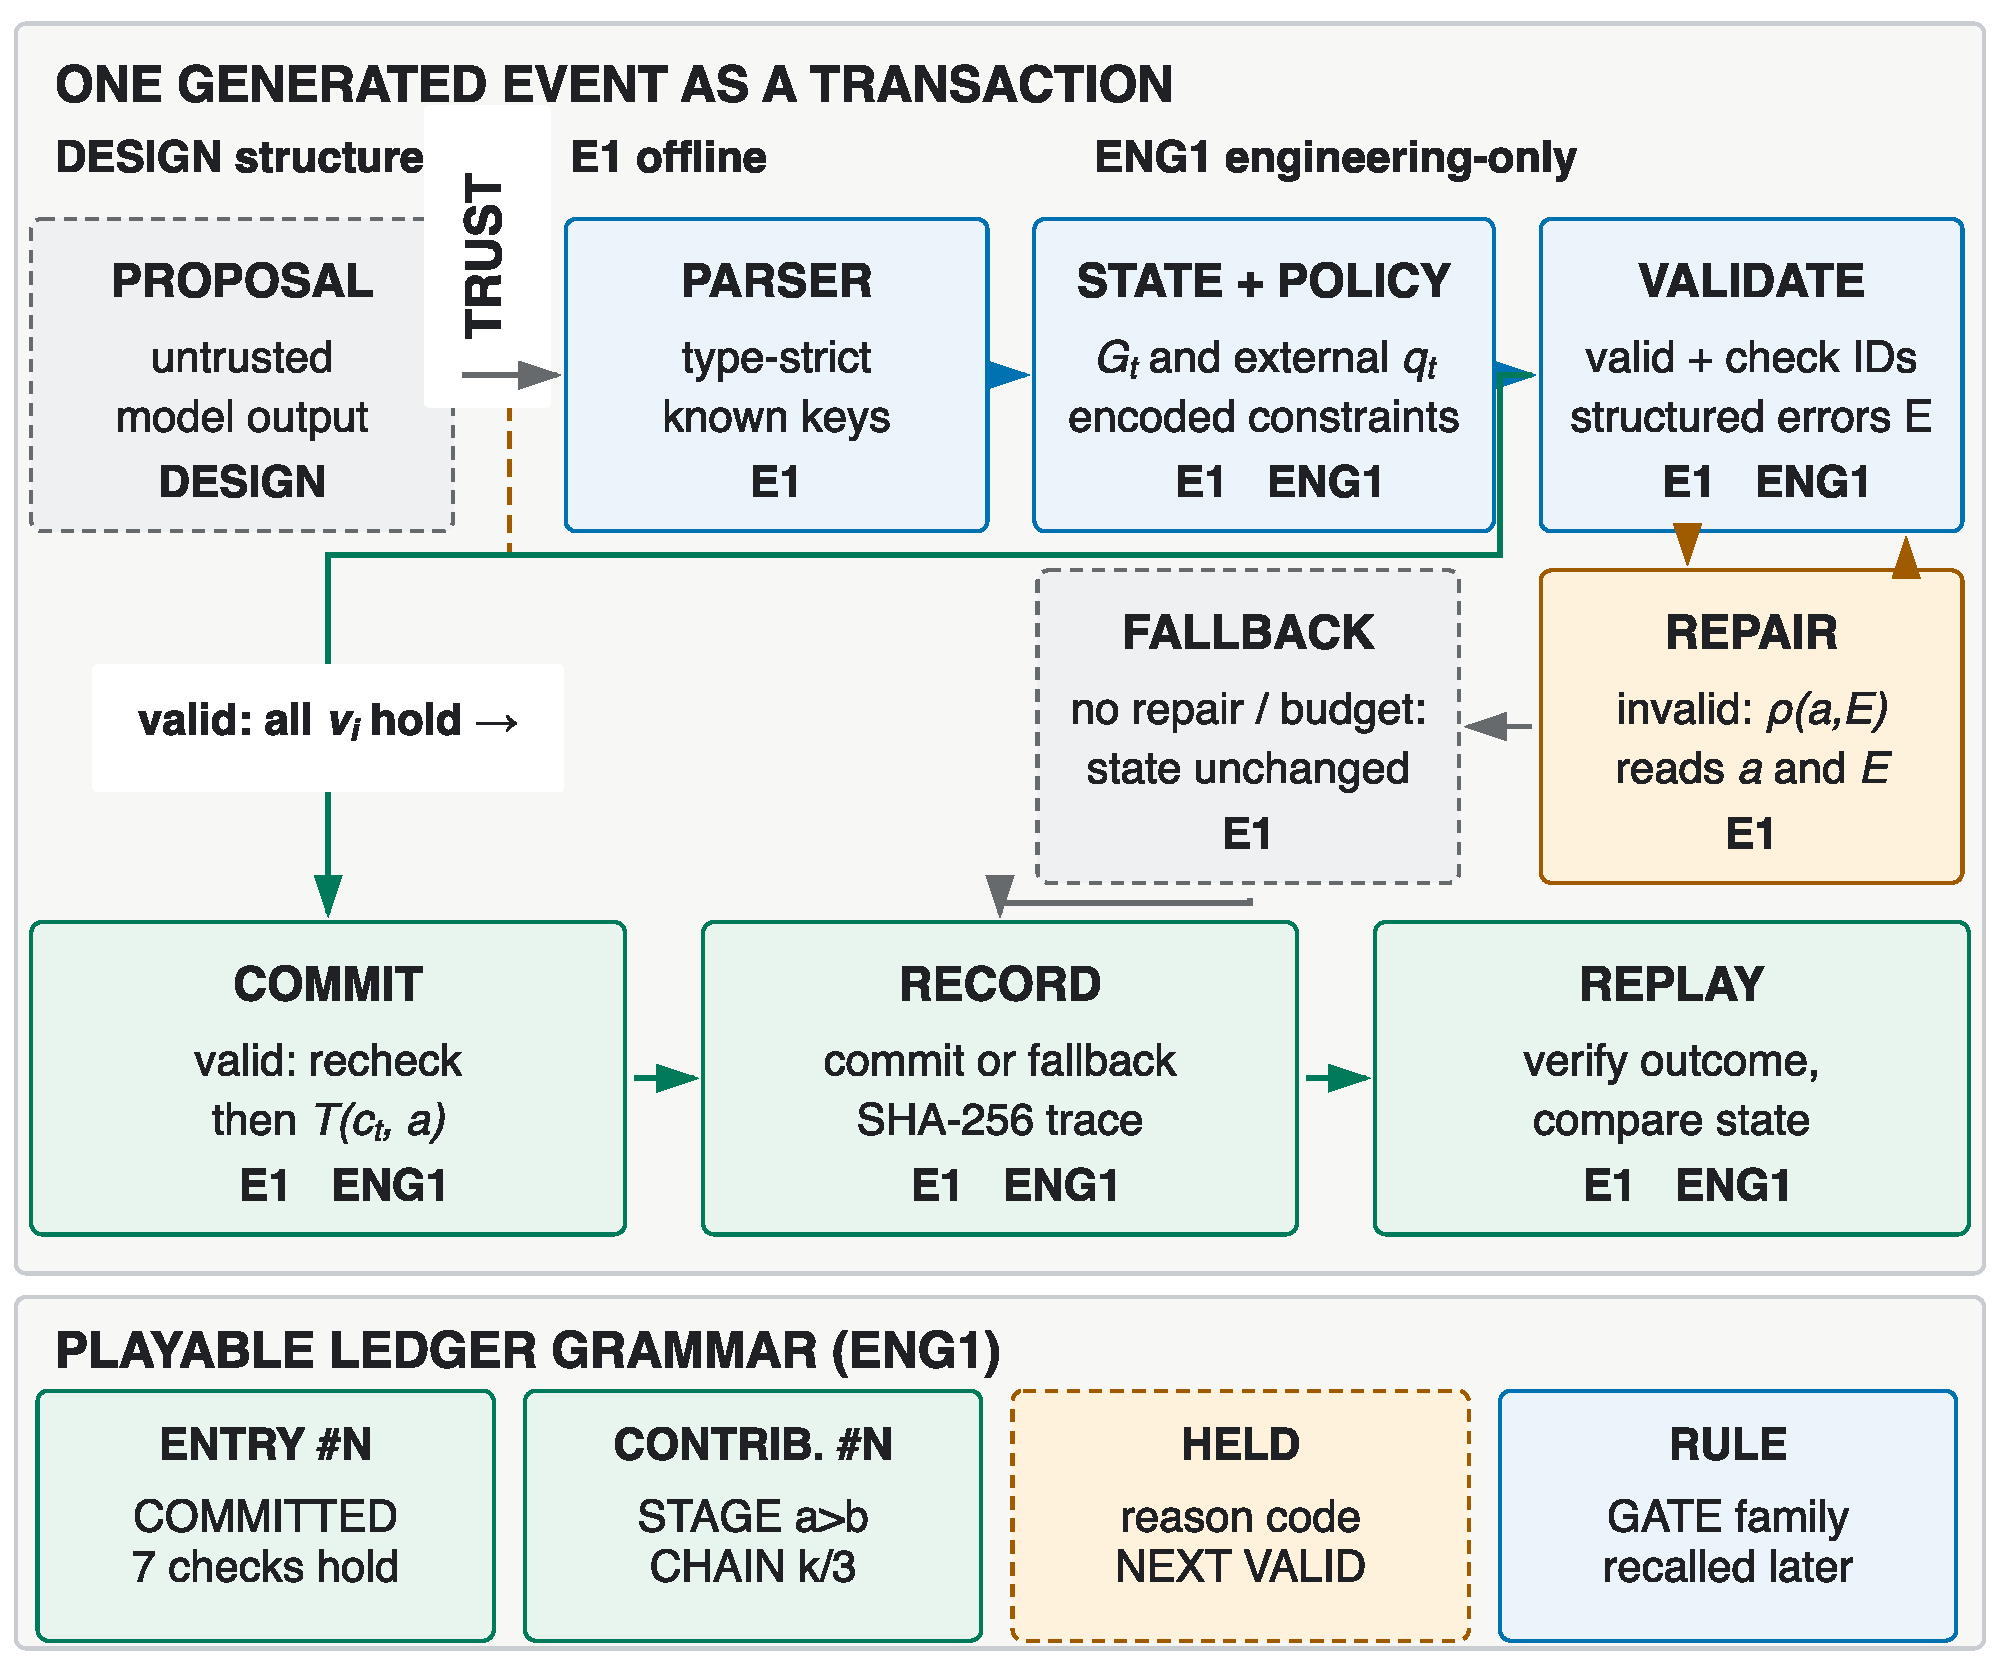
\includegraphics[width=0.92\textwidth]{../../figures/fig_architecture.pdf}
  \caption{Policy and state $c_t$ gate proposals; errors feed bounded $\rho$ or unchanged fallback before revalidated commit and replay.}
  \label{fig:architecture}
\end{figure}

\section{Problem Definition and Guarantee Boundary}\label{sec:problem}
In $c_t=(G_t,q_t)$, $G_t$ denotes the typed game snapshot (locations, reachable locations, object placements, inventory, facts, NPC knowledge, and quest stage) and $q_t$ contains externally authored action-policy, disclosure, and quest-stage constraints. Predicates neither reconstruct history $h_{<t}$ nor mutate $q_t$, and retrieval outputs or affect scores carry zero write authority.

After strict schema parsing of an untrusted proposal $a_t$, the validator runs seven deterministic predicates and returns \texttt{Validation}\allowbreak\texttt{Result}(\allowbreak$\mathrm{valid},E_t,C_{\mathrm{run}}$):
\begin{equation}
\begin{aligned}
V(c_t,a_t)&=(\mathrm{valid},E_t,C_{\mathrm{run}}),\\
\boldsymbol{v}&=(v_{\mathrm{policy}},v_{\mathrm{pre}},v_{\mathrm{reach}},\\
&\qquad v_{\mathrm{know}},v_{\mathrm{disc}},v_{\mathrm{elig}},v_{\mathrm{stage}})\in\{0,1\}^{7},
\end{aligned}
\end{equation}
where $\mathrm{valid}\equiv\bigwedge_{i=1}^{7}(v_i=1)$ and $E_t$ records typed error codes, entities, reasons, and repair hints. Canonical state updates only when all seven predicates pass:
\begin{equation}
c_{t+1}=\begin{cases}
T(c_t,a_t), & \bigwedge_{i=1}^{7}(v_i=1),\\
c_t, & \text{otherwise.}
\end{cases}
\label{eq:transition}
\end{equation}

\subsection{Schema Validity, Authorization, and Goal Success}\label{sec:authorization-sets}
Fix the pre-action state $c_t$, authored policy, and strict schema. Let $\SchemaSet$ be the set of schema-valid candidates; we separate authorization from goal attainment:
\begin{equation}
\begin{aligned}
\AcceptSet(c_t)&=\{a\in\SchemaSet:V(c_t,a).\mathrm{valid}\},\\
\GoalSet(c_t)&=\{a\in\SchemaSet:\operatorname{Goal}(T(c_t,a))\},\\
\HitSet(c_t)&=\AcceptSet(c_t)\cap\GoalSet(c_t)\subseteq\AcceptSet(c_t)\subseteq\SchemaSet.
\end{aligned}
\end{equation}
A schema-valid candidate that declares a forbidden fact falls outside $\AcceptSet$, whereas a permitted observation action can lie inside $\AcceptSet$ yet outside $\GoalSet$. Knowledge and disclosure permission are independent inputs: an NPC can know \texttt{keeper\_\allowbreak secret} at both stage $0$ and stage $1$ while disclosure is forbidden at stage $0$ and permitted at stage $1$.

\subsection{Formal Security Theorems for Invariants I1--I4}\label{sec:formal-proofs}
Under Eq.~\eqref{eq:transition} and strict parser \texttt{parse\_}\allowbreak\texttt{candidate\_}\allowbreak\texttt{mapping}, invariants \textbf{I1--I4} hold as conditional structural theorems over any finite encoded state $c_t=(G_t,q_t)$, repair budget $K\in\mathbb{Z}_{\geq 0}$, and returning callbacks:

\noindent\textbf{Theorem 1 (I1: State-Preservation Safety).} \emph{If the initial candidate fails strict parsing or all $K{+}1$ candidates yield $V(c_t,a^{(j)}).\mathrm{valid}=\mathrm{false}$, then $c_{t+1}=c_t$ and committed effects are empty.}
\par\noindent\textit{Proof.} \texttt{parse\_}\allowbreak\texttt{candidate\_}\allowbreak\texttt{mapping} rejects malformed proposals prior to commit; in Fig.~\ref{alg:commit}, $\operatorname{Commit}$ is reachable only on $\mathrm{ok}=\mathrm{true}$, while $j=K$ invokes $\operatorname{Fallback}(c_t)$ returning $c_t$ untouched by Eq.~\eqref{eq:transition}. \hfill$\square$

\noindent\textbf{Theorem 2 (I2: Bounded Termination and State-Blind Anti-Laundering Repair).} \emph{For any finite $K{\geq}0$ and returning callbacks, the loop executes at most $K{+}1$ validator calls, revalidates $V(c_t,a^{(j)})$ immediately prior to mutation, and never alters \texttt{WorldState}-dependent authorization classes under $\rho$.}
\par\noindent\textit{Proof.} Loop counter $j$ starts at $0$, checks $j=K$ before incrementing, and halts on $\mathrm{ok}=\mathrm{true}$ or $j=K$, bounding $V$ calls by $K{+}1$. By Table~\ref{tab:rho-rules}, $\rho(a,E)$ inspects only $(a,E)$ without reading \texttt{WorldState} and maps \texttt{UNKNOWN\_}\allowbreak\texttt{ACTION\_}\allowbreak\texttt{TYPE}, \texttt{UNREACHABLE\_}\allowbreak\texttt{REQUIRED\_}\allowbreak\texttt{OBJECT}, \texttt{NPC\_}\allowbreak\texttt{KNOWLEDGE\_}\allowbreak\texttt{VIOLATION}, \texttt{NPC\_}\allowbreak\texttt{DIS\-CLOSURE\_}\allowbreak\texttt{KNOW\-LEDGE\_}\allowbreak\texttt{VIO\-LATION}, \texttt{FORBIDDEN\_}\allowbreak\texttt{DISCLOSURE}, \texttt{QUEST\_}\allowbreak\texttt{STAGE\_}\allowbreak\texttt{VIOLATION}, and \texttt{QUEST\_}\allowbreak\texttt{STAGE\_}\allowbreak\texttt{REGRESSION} to identity while dropping same-field conflicts. \hfill$\square$

\noindent\textbf{Theorem 3 (I3: Policy-Bounded Mutation).} \emph{Every committed state transition satisfies all seven predicates $v_1\dots v_7$ and applies only effects permitted by \texttt{ActionPolicy.}\allowbreak\texttt{allowed\_}\allowbreak\texttt{effects}.}
\par\noindent\textit{Proof.} Strict parsing freezes the 12 \texttt{CANDIDATE\_}\allowbreak\texttt{FIELDS}; $v_{\mathrm{policy}}{=}1$ verifies effect membership in \texttt{allowed\_}\allowbreak\texttt{effects} and $T$ writes no undeclared keys. \hfill$\square$

\noindent\textbf{Theorem 4 (I4: Deterministic Semantic Replay).} \emph{Given ordered hash-chained transition records with \texttt{allow\_}\allowbreak\texttt{defaults=false} parsing and frozen $(V,T)$, replaying proposals from $c_0$ uniquely reconstructs $c_T$ and detects any single-step tampering via SHA-256 chain mismatch.}
\par\noindent\textit{Proof.} Both $V$ and $T$ are pure deterministic functions of $(c_t,a_t)$, and each record hashes $(\mathrm{hash}(c_t),\allowbreak a_t,\allowbreak V(c_t,a_t),\allowbreak\mathrm{hash}(c_{t+1}))$; inductive agreement from $c_0$ yields $\mathrm{hash}(c'_T)=\mathrm{hash}(c_T)$. \hfill$\square$

\section{TRACE-RPG Architecture and Algorithms}\label{sec:arch}
Models and adapters submit typed candidate JSON via direct HTTPS structured decoding or constrained prompts, the strict parser rejects unknown keys and ambiguous types, and a versioned bridge exchanges observations, candidates, validation errors, repairs, and commits (Fig.~\ref{fig:architecture}, Table~\ref{tab:validators}). An eight-role read-only ontology view (\texttt{World}, \texttt{Actor}, \texttt{Knowledge}, \texttt{Fact}, \texttt{Policy}, \texttt{Quest}, \texttt{Action}, \texttt{Trace}) links source declarations to executed predicates without write authority.

\subsection{Multi-Hop Datalog Closure and Comparative Safety Baselines}\label{sec:multihop-baselines}
When narrative secrets derive through multi-step premise chains or role hierarchies up to depth $d$, flat 1-hop gating fails to detect indirect leaks. The core \texttt{nesy\_\allowbreak game.\allowbreak multihop} module evaluates a frozen declarative \texttt{MultihopOntologySpec} containing \texttt{role\_parents}, \texttt{fact\_implications}, \texttt{forbidden\_by\_role}, and \texttt{min\_stage\_by\_fact}. Calling \texttt{compute\_datalog\_closure} computes the bottom-up semi-naive fixpoints over role inheritance $\mathcal{R}^*(u)$ and fact implications $\mathcal{F}^*(S)$ up to arbitrary finite depth $d$:
\begin{equation}
\mathcal{F}^*(S)=\operatorname{lfp}\Big(X\mapsto S\cup\bigcup_{f\in X}\texttt{fact\_implications}(f)\Big),
\end{equation}
and propagates role prohibitions $\bigcup_{r\in\mathcal{R}^*(u)}\texttt{forbidden\_by\_role}(r)$ plus dynamic state prohibitions before evaluating $v_{\mathrm{know}}, v_{\mathrm{disc}}, v_{\mathrm{stage}}$ in \texttt{validate\_\allowbreak candidate\_\allowbreak multihop}. To situate this boundary against established safety paradigms over the identical \texttt{WorldState} contract without external neural RL policy training or separate server deployments, our package implements two controlled in-engine proxy comparators: (i)~\textbf{Safe-RL Action Masking} (\texttt{evaluate\_\allowbreak action\_\allowbreak mask\_\allowbreak shield}, following~\cite{alshiekh2018shield}), which enforces declared action-type, reachability, and 1-hop precondition masks over observable action tuples while omitting transitive role/fact closure; and (ii)~\textbf{NeMo-style Colang Output Rail} (\texttt{evaluate\_\allowbreak dialog\_\allowbreak rail\_\allowbreak filter}, following~\cite{rebedea2023nemo}), which filters surface secret strings and direct 1-hop dialogue policies over emitted utterances without multi-hop state closure.

\begin{table}[!tbp]
\caption{Encoded Seven-Predicate Validator Boundary}
\label{tab:validators}
\centering
\footnotesize
\begin{tabularx}{\columnwidth}{@{}>{\raggedright\arraybackslash}p{0.25\columnwidth}>{\raggedright\arraybackslash}X>{\raggedright\arraybackslash}p{0.17\columnwidth}@{}}
\toprule
\textbf{Predicate} & \textbf{Rejects} & \textbf{On failure} \\
\midrule
Action policy & unknown action/type; omitted preconditions/effects; disallowed effects & unchanged \\
Precondition & absent or false requirement & unchanged \\
Reachability & inaccessible target object & unchanged \\
NPC knowledge & used/disclosed fact absent from actor knowledge & unchanged \\
Disclosure & declared or Datalog-derived forbidden fact & unchanged \\
Quest stage & required stage (incl.\ derived min-stage) above current stage & unchanged \\
Stage monotonicity & regressive quest-stage mutation & unchanged \\
\bottomrule
\end{tabularx}
\end{table}

\begin{figure}[!tbp]
\centering
\footnotesize
\begin{tabular}{@{}rl@{}}
1: & $a\leftarrow\operatorname{Propose}(c)$; $j\leftarrow0$ \\
2: & \textbf{repeat} \\
3: & \quad $(\mathrm{ok},E)\leftarrow V(c,a)$; $\operatorname{Record}(a,E)$ \\
4: & \quad \textbf{if} $\mathrm{ok}$ \textbf{then assert} $V(c,a).\mathrm{ok}$; \textbf{return} $\operatorname{Commit}(c,a)$ \\
5: & \quad \textbf{if} $j=K$ \textbf{then return} $\operatorname{Fallback}(c)$ \\
6: & \quad $a\leftarrow\operatorname{Repair}(c,a,E)$; $j\leftarrow j+1$ \\
7: & \textbf{until terminal}
\end{tabular}
\caption{Validate--Repair--Commit records at most $K+1$ candidate attempts and revalidates before mutation.}
\Description{Pseudocode of the Validate-Repair-Commit loop bounding validator calls to K+1 and revalidating prior to commit.}
\label{alg:commit}
\end{figure}

Guided repair $\rho(a,E)=a\oplus\bigcup_{e\in E}\delta(e)$ (Fig.~\ref{alg:commit}, Table~\ref{tab:rho-rules}) and \texttt{execute\_\allowbreak with\_\allowbreak multihop\_\allowbreak repair} inspect only candidate $a$ and typed errors $E$, never \texttt{WorldState}, preventing state laundering on authorization faults. Transition records chain unkeyed SHA-256 hashes over prior state, candidate, validation outcome, and recomputed final state for bit-exact semantic replay.

\begin{table}[!tbp]
\caption{Per-Error-Class Edits of Guided Repair $\rho(a,E)$}
\label{tab:rho-rules}
\centering
\footnotesize
\begin{tabularx}{\columnwidth}{@{}>{\raggedright\arraybackslash}X>{\raggedright\arraybackslash}X@{}}
\toprule
\textbf{Validator error class} & \textbf{Edit $\delta(e)$ on candidate $a$} \\
\midrule
Policy precondition / effect omission & insert named predicate or effect \\
Policy effect violation & drop disallowed effect \\
Unsatisfied precondition & drop named predicate \\
Unauthorized stage mutation & clear \texttt{quest\_stage\_effect} \\
Unknown action; reachability, knowledge, disclosure, or stage classes & no-op (prevents state laundering) \\
\bottomrule
\end{tabularx}
\end{table}

\section{Benchmark Suite Composition, Curation, and Maintenance}\label{sec:db-composition}
\system{} is packaged as a standalone, zero-network-reproducible benchmark suite built around the frozen core (\texttt{src/nesy\_game/*.py}, 20/20 SHA-256 hashes unchanged) and \texttt{nesy\_game.multihop}. Following Gebru et al.~\cite{gebru2021datasheets} (\texttt{DATASHEET\_v5.md}) and ML Commons Croissant~1.0~\cite{akhtar2024croissant} (\texttt{croissant\_trace\_rpg\_benchmark\_v5.json}), the v5 archival bundle (\texttt{neurips-db-supplemental-benchmark.zip}, 55 files, \texttt{CHECKSUMS.sha256} 54/54 verified, zero PII/IP/secret leaks) indexes \textbf{26 SHA-256-verified \texttt{FileObject} artifacts} (v2: 12, v3: 17, v4: 22, v5: 26) under dual \textbf{MIT} (verification harnesses and oracle code) and \textbf{CC BY 4.0} (traces, structured quest specs, and evaluation receipts) licenses. No web scraping or user-sourced text appears anywhere in the benchmark.

\begin{table}[!tbp]
\caption{Benchmark Suite Composition Across Determinism, Engine Replay, and Attested API Cohorts (Croissant~1.0 v5: 26/26 FileObjects)}
\label{tab:phase5-db-comp}
\centering
\scriptsize
\setlength{\tabcolsep}{3pt}
\begin{tabularx}{\columnwidth}{@{}>{\raggedright\arraybackslash}p{0.27\columnwidth}c>{\raggedright\arraybackslash}X@{}}
\toprule
\textbf{Suite Partition} & \textbf{Size} & \textbf{Schema, Provenance, and Isolation Rule} \\
\midrule
Deterministic Finite-Graph & 1,664 + 48 & 32 graph configs $\times$ 13 candidates $\times$ 4 arms + surface sentinels; BFS oracle. \\
Extended Audits (\textbf{A1}--\textbf{A4}, \textbf{B}) & 1,408 + 1,600t & Multi-error $K{\le}3$, $N{\le}2000$ scaling, 4,656 faults, Godot soak, 88 EN/KO B. \\
Datalog Depth Scaling (\textbf{P9}) & 480 cases & Procedural $R{\in}\{8..64\}\times d{\in}\{1..5\}$ DAGs; bottom-up fixpoint + BFS. \\
Phase-5 Closed-Loop MAS (\textbf{P15}) & 105 ep & 3 Claude~5.5 tiers $\times$ 5 worlds $\times$ 7 independent arms; \texttt{output\_config}. \\
Phase-5 API Factorial+Godot (\textbf{P16}) & 60 + 21 ep & Attested API (no \texttt{temp}) + Godot~4.7.1; non-pooled w/ 0/180 \texttt{20261103}. \\
Phase-5 Unified Escape (\textbf{P17}) & 540 evals & 180 EN/KO cases $\times$ 3 Claude~5.5 tiers; 0 deterministic short-circuits. \\
Phase-4 Cross-Family (\textbf{P11}--\textbf{P14}) & 30 / 90 / 42 / 720 & Unseeded CLI (Sonnet~5.5, GPT-OSS~120B, Gemini~4~Hydrogen/3.8~Flash). \\
Held-Out / Unrun Templates & \texttt{N=0} / 0/180 & Blinded \texttt{TR01--TR06} (\texttt{AWAITING\_HUMAN\_RATERS}) \& frozen \texttt{20261103} excluded. \\
\bottomrule
\end{tabularx}
\end{table}

\textbf{Curation, attestation, and maintenance.} Deterministic tasks derive from symbolic quest state machines (${\le}8$ rooms, ${\le}3$ actors) and procedural $R{\le}64, d{\le}5$ Datalog graphs paired with EN/KO utterances. Direct HTTPS Phase-5 traces log \texttt{served\_model}, SHA-256-hashed message/request IDs, token counts, and HTTP latency under strict structured-JSON schemas (\texttt{temperature} omitted where deprecated on Claude~5.5); every parse/HTTP failure stays in full denominators. Crucially, the blinded 36-item packet \texttt{TR01--TR06} (\texttt{N=0}) and historical unrun \texttt{prospective-pilot-20261103} (\texttt{0/180}) are strictly quarantined from machine leaderboards. Standalone \texttt{python3 reproduce\_benchmark.py} re-verifies all 54 checksums, 26 Croissant digests, Theorem~1--4 properties, and Datalog scaling offline in $<5$\,s.

\section{Reproducible Benchmark Leaderboards}\label{sec:eval}
\subsection{Cross-Track Shielding, Repair, Godot, and Escape Results}\label{sec:phase4-compact}
We evaluate all baseline gates, external comparators (\textbf{Safe-RL Action Masking}~\cite{alshiekh2018shield} and \textbf{NeMo-style Colang Output Rails}~\cite{rebedea2023nemo}), and neural models on unified replay-verified tracks (Table~\ref{tab:phase4-compact}).

\begin{table}[!tbp]
\caption{Cross-Track Benchmark Leaderboard: Deterministic (\textbf{P9}), Attested Claude~5.5 API (\textbf{P15}--\textbf{P17}), and 3-Family CLI (\textbf{P11}--\textbf{P14})}
\label{tab:phase4-compact}
\centering
\scriptsize
\setlength{\tabcolsep}{2.5pt}
\begin{tabularx}{\columnwidth}{@{}>{\raggedright\arraybackslash}p{0.27\columnwidth}>{\raggedright\arraybackslash}X@{}}
\toprule
\textbf{Benchmark Track} & \textbf{Measured Leaderboard Result (95\% Wilson CI; $Q$ / McNemar $p$)} \\
\midrule
Boundary \& Audits (0-LLM) & Semantic gates \textbf{0/416} unsafe (vs.\ schema 260/416); $\rho$ 128/260 repairs; Godot \textbf{A4} 1,600/1,600 ticks, p95 0.708\,ms; \textbf{P1} 120-case \textbf{100\%} vs.\ 50.83\%. \\
\textbf{P9} Datalog Scaling (480) & \texttt{flat\_1hop}: 46.67\% (256 leaks); \texttt{2hop}: 60.00\% (192); \texttt{nesy\_game.multihop}: \textbf{100.0\% [99.2, 100]} at $\le$7.12\,$\mu$s median ($Q{=}1100.19$). \\
\textbf{P15} Closed-Loop MAS (105) & Independent 5-turn trajectories (\textbf{105/105} replays): Safe-RL proxy~\cite{alshiekh2018shield} 0/15 goals, 16/61 unsafe; NeMo proxy~\cite{rebedea2023nemo} 1/15, 15/61; flat 12/15, 4/66; \texttt{multihop\_k0} 13/15, \textbf{15/15} zl, \textbf{0/69}; \texttt{rho\_k2} 14/15 ($\rho_{\mathrm{rep}}{=}0$ per Thm.~2), \textbf{15/15} zl, \textbf{0/68}; \textbf{hybrid} \textbf{15/15 (100\%)}, 15/15 zl, \textbf{0/63} ($Q_{\mathrm{goal}}{=}68.71$). \\
\textbf{P16} API Factorial+Godot (81) & \textbf{P16A}: \texttt{general\_rule} 0/30 goals, 22/30 zl, 9 unsafe vs.\ \texttt{ontology\_multihop} \textbf{30/30} zl ($p{=}0.0078$), 11/30 goals (Opus 8/10), \textbf{0} unsafe. \textbf{P16B}: \textbf{21/21} Godot replays, \textbf{0/21} leaks, 13/15 5-world + \textbf{6/6} \texttt{SealedLighthouse} hash matches. \\
\textbf{P17} Unified Escape (540) & 0 short-circuits, $\kappa{=}\mathbf{0.8813}$: \texttt{haiku} 29/36 exp / \textbf{70/72} para / 0\% FRR / $F_1{=}\mathbf{0.957}$; \texttt{sonnet} 19/36 / 70/72 / $0.904$; \texttt{opus} 25/36 / 68/72 / $0.925$ (Stage-1 \texttt{id\_only} 36/36). \\
\textbf{P11}--\textbf{P14} 3-Family CLI & GPT-OSS~120B + Hydrogen~4 + Sonnet: \textbf{P11} \textbf{30/30} zl, \textbf{0/79} unsafe ($Q{=}118.93$); \textbf{P12} 27 faults $\rho_{K=2}$ \textbf{27/27} (0 tok) vs.\ Blind/Aware LLM 26/27 (530k--542k tok, $p{=}1.0$); \textbf{P13} \textbf{42/42} Godot replays; \textbf{P14} $\kappa{=}\mathbf{0.9367}$. \\
\bottomrule
\end{tabularx}
\end{table}

Together, \textbf{P9} and \textbf{P15}--\textbf{P17} demonstrate why benchmarked runtime gating needs both symbolic closure and semantic text inspection: Safe-RL masking~\cite{alshiekh2018shield} and NeMo-style rails~\cite{rebedea2023nemo} fail 14/15 episodes under multi-hop dependency chains (\textbf{P15}), flat general rules suffer 9 unsafe commits across Sonnet and Opus (\textbf{P16A}), deterministic $\rho_{K=2}$ removes $>500\text{k}$ repair tokens per 27 faults at $p{=}1.0$ accuracy parity (\textbf{P12}), and unified Claude~5.5 Stage-2 verifiers still miss explicit unhinted IDs inside prose (19--29/36 in \textbf{P17}), confirming strict Stage-1 + Stage-2 complementarity.

\FloatBarrier
\section{Threats to Validity, Limitations, and Conclusion}\label{sec:conclusion}
\textbf{Limitations and threats to validity.} Four explicit boundaries constrain the scope of our claims across deterministic audits, cross-family CLI trials, and Phase-5 direct Anthropic API experiments:
(1)~\emph{API decoding, proxy comparators, and unseeded CLI runs:} Phase-5 direct HTTPS calls to Anthropic \texttt{claude-haiku-5-5}, \texttt{claude-sonnet-5-5}, and \texttt{claude-opus-5-5} use native structured outputs (\texttt{output\_config.json\_schema}) with \texttt{temperature} omitted because Claude~5.5 rejects \texttt{temperature} as deprecated, evaluate \textbf{P15} on a single API vendor under a turn-scheduled 2-NPC interaction protocol (complemented by 3-family CLI negotiation in \textbf{P11}) against controlled in-engine Safe-RL/NeMo proxy comparators, whereas Phase-4 CLI tracks (\textbf{P11}--\textbf{P14}: GPT-OSS~120B, Gemini~4~Hydrogen, 3.8~Flash, and CLI Sonnet fallback) reflect unseeded decoding; all API and CLI parse failures remain inside full denominators;
(2)~\emph{Non-pooled prospective cohorts:} the historical 180-unit pre-registered protocol (\texttt{prospective-pilot-20261103}) remains \texttt{0/180} (\texttt{NOT\_RUN/BLOCKED}) and untouched rather than pooled with Phase-5 attested \textbf{P16};
(3)~\emph{Symbolic quest scope:} our five quest worlds (${\le}8$ rooms, ${\le}3$ actors), production \texttt{Sealed\allowbreak Lighthouse\allowbreak Machine}, and $R{\le}64, d{\le}5$ Datalog graphs isolate symbolic runtime authorization and Godot~4.7.1 state integrity rather than open-world 3D physics or free-form combat; and
(4)~\emph{Zero human-rater claims ($N{=}0$):} the blinded 36-item packet \texttt{TR01--TR06} (\texttt{AWAITING\_}\allowbreak\texttt{HUMAN\_}\allowbreak\texttt{RATERS}) contains zero synthetic labels, so human usability, immersion, player enjoyment, and human Krippendorff~$\alpha$ remain unmeasured future work.

\textbf{Conclusion.} \system{} decouples neural proposal from canonical engine commit via a seven-predicate validator, semi-naive bottom-up Datalog closure (\texttt{nesy\_game.multihop}), state-blind counterexample repair $\rho(a,E)$, and SHA-256 hash-chained semantic replay (Theorems~1--4 for \textbf{I1--I4}). Beyond deterministic scaling to $R{=}64, d{=}5$ (\textbf{P9}: 480/480 at $\le$7.12\,$\mu$s, $Q{=}1100.19$), attested direct Anthropic API runs spanning Haiku, Sonnet, and Opus~5.5 confirm \textbf{0} unsafe commits across 105 independent 5-turn closed-loop episodes (\textbf{P15}: \textbf{15/15} zero-leak across every \texttt{nesy\_game.multihop} arm and \textbf{15/15} safe goals via hybrid $\rho{+}\text{LLM}_{K=1}$, empirically confirming Theorem~2 no-op safety with $\rho_{\mathrm{repairs}}{=}0$ on 28 state-dependent rejections vs.\ Safe-RL proxy masking 0/15 and NeMo-style proxy rails 1/15, $Q{=}68.71$), while deterministic $\rho$ executes \textbf{22} live runtime repairs in 60 prospective factorial episodes (\textbf{P16A}: \textbf{30/30} zero-leak and 11/30 goals under \texttt{ontology\_multihop} vs.\ 22/30 and 0/30 under \texttt{general\_rule}), \textbf{27/27} zero-token repairs on matched policy+stage faults (\textbf{P12}), and 128/260 finite-graph repairs alongside \textbf{21/21} Godot~4.7.1 replays (\textbf{P16B}: 6/6 production \texttt{EXACT\_TERMINAL\_HASH}, 0/21 leaks). Combined with cross-family CLI generalization (\textbf{P11}--\textbf{P14}: 0/79 and 0/84 unsafe commits, 42/42 Godot replays), unified Stage-2 EN/KO escape (\textbf{P17}: 540 fresh evals, Fleiss' $\kappa{=}0.8813$, 0\% FRR), and Croissant~1.0 v5 (26/26 SHA-256 digests + \texttt{DATASHEET\_v5.md}), \system{} establishes an auditable engineering and benchmark foundation for safe agentic games.

\section*{Ethical and Artifact Statement}
Large language models assisted with prose drafting, auxiliary harnesses, and test generation; all theorems, citations, API traces, statistics, and deterministic replays were audited with zero fabricated human ratings ($N{=}0$). Code and reproducible artifacts: \RepoURL.


\FloatBarrier
\bibliographystyle{plainnat}
\bibliography{../../references,../_shared/venue_extra}

\clearpage
\section*{NeurIPS Paper Checklist}
\begin{enumerate}
\item {\bf Claims}
    \item[] Question: Do the main claims made in the abstract and introduction accurately reflect the paper's contributions and scope?
    \item[] Answer: \answerYes{}
    \item[] Justification: All deterministic counts, attested Phase-5 direct Anthropic API tracks (\textbf{P15}--\textbf{P17}, retaining all parse/API counts), confound-free Phase-4 3-family denominators (\textbf{P11}--\textbf{P14}), external Safe-RL~\cite{alshiekh2018shield} / NeMo~\cite{rebedea2023nemo} comparators, and unexecuted cohorts (0/180 \texttt{20261103}; $N{=}0$ human raters) match JSON receipts in \texttt{research/green-supplements/}.
\item {\bf Limitations}
    \item[] Question: Does the paper discuss the limitations of the work performed by the authors?
    \item[] Answer: \answerYes{}
    \item[] Justification: Claude~5.5 omitted \texttt{temperature} (\texttt{output\_config.json\_schema}), unseeded CLI revisions/seeds (\textbf{P11}--\textbf{P14}), retained parse failures, historical 0/180 unexecuted pilot, finite symbolic world scope, and $N{=}0$ human evaluation (\texttt{AWAITING\_}\allowbreak\texttt{HUMAN\_}\allowbreak\texttt{RATERS}) are detailed in Sec.~\ref{sec:conclusion}.
\item {\bf Theory assumptions and proofs}
    \item[] Question: For each theoretical result, does the paper provide the full set of assumptions and a complete (and correct) proof?
    \item[] Answer: \answerYes{}
    \item[] Justification: Sec.~\ref{sec:formal-proofs} states exact preconditions ($c_t$, finite $K\in\mathbb{Z}_{\geq 0}$, strict \texttt{parse\_}\allowbreak\texttt{candidate\_}\allowbreak\texttt{mapping}, returning callbacks) and proves Theorems~1--4 for invariants \textbf{I1--I4}.
\item {\bf Experimental result reproducibility}
    \item[] Question: Does the paper fully disclose all the information needed to reproduce the main experimental results of the paper to the extent that it affects the main claims and/or conclusions of the paper (regardless of whether the code and data are provided or not)?
    \item[] Answer: \answerYes{}
    \item[] Justification: Deterministic \texttt{nesy\_game.multihop} verifier modules, $R{\le}64, d{\le}5$ Datalog oracle parameters, direct HTTPS \texttt{output\_config.json\_schema} schemas, $(a,E)$ repair prompts, and unified escape prompts are disclosed in Secs.~\ref{sec:arch}--\ref{sec:eval}.
\item {\bf Open access to data and code}
    \item[] Question: Does the paper provide open access to the data and code, with sufficient instructions to faithfully reproduce the main experimental results, as described in supplemental material?
    \item[] Answer: \answerYes{}
    \item[] Justification: \ifanonymoussubmission The self-contained OpenReview/double-anonymous supplemental archive (\texttt{neurips-db-supplemental-benchmark.zip}, 55 files, \texttt{CHECKSUMS.sha256} 54/54 verified, 0~PII/secret leaks) packages all Phase-1--5 JSON receipts, \texttt{DATASHEET\_v5.md}~\cite{gebru2021datasheets}, Croissant~1.0~\cite{akhtar2024croissant} v2--v5 (12/12, 17/17, 22/22, and 26/26 SHA-256 digests), MIT/CC-BY-4.0 \texttt{LICENSE}, core \texttt{nesy\_game.multihop}, and zero-network \texttt{reproduce\_benchmark.py} passing in $<5$\,s.\else Repository, \texttt{DATASHEET\_v5.md}~\cite{gebru2021datasheets}, Croissant~1.0~\cite{akhtar2024croissant} v2--v5 (26/26 SHA-256 digests), and standalone \texttt{reproduce\_benchmark.py} are available at \RepoURL\ and in the 55-file supplemental benchmark archive.\fi
\item {\bf Experimental setting/details}
    \item[] Question: Does the paper specify all the training and test details (e.g., data splits, hyperparameters, how they were chosen, type of optimizer, etc.) necessary to understand the results?
    \item[] Answer: \answerYes{}
    \item[] Justification: Graph dimensions, 5-world strata, $R{\le}64, d{\le}5$ Datalog parameters, Safe-RL/NeMo definitions, Haiku/Sonnet/Opus~5.5 direct API settings (omitted deprecated \texttt{temperature}), $K\in\{0,1,2\}$ repair budgets, and 3-domain EN/KO splits are specified in Secs.~\ref{sec:db-composition}--\ref{sec:eval}.
\item {\bf Experiment statistical significance}
    \item[] Question: Does the paper report error bars suitably and correctly defined or other appropriate information about the statistical significance of the experiments?
    \item[] Answer: \answerYes{}
    \item[] Justification: Sec.~\ref{sec:phase4-compact} and Table~\ref{tab:phase4-compact} report 95\% Wilson CIs, Cochran's $Q$ ($Q{=}1100.19$ for \textbf{P9}; $Q_{\mathrm{goal}}{=}68.71$, $Q_{\mathrm{zl}}{=}71.65$ for \textbf{P15}; $Q{=}118.93, 281.23$ for \textbf{P11}--\textbf{P12}), exact two-sided McNemar $p$-values (\textbf{P15} $p{\le}1.22{\times}10^{-4}$; \textbf{P16A} $p{=}0.00781, 9.77{\times}10^{-4}$; \textbf{P12} $p{=}1.0$), and Fleiss' $\kappa{=}0.8813$ (\textbf{P17}) / $0.9367$ (\textbf{P14}).
\item {\bf Experiments compute resources}
    \item[] Question: For each experiment, does the paper provide the computer resources (type of compute workers, memory, time of execution, etc.) required to reproduce the experiments?
    \item[] Answer: \answerYes{}
    \item[] Justification: Audits \textbf{A2}/\textbf{A4}/\textbf{P9} report CPU latencies ($\le$7.12\,$\mu$s p50 at $R{=}64$), and live API/CLI traces record full tokens and latencies (\textbf{P15} 1.05M tok; \textbf{P16A} 674k tok; \textbf{P16B} 169k tok + Godot ms vs.\ API s; \textbf{P17} 359k tok; \textbf{P12} 530k/542k tok vs.\ 0 for $\rho$).
\item {\bf Code of ethics}
    \item[] Question: Does the research conducted in the paper conform, in every respect, with the NeurIPS Code of Ethics?
    \item[] Answer: \answerYes{}
    \item[] Justification: Sec.~\ref{sec:conclusion} covers AI-usage disclosure, zero fabricated human labels, and safety boundaries.
\item {\bf Broader impacts}
    \item[] Question: Does the paper discuss both potential positive societal impacts and negative societal impacts of the work?
    \item[] Answer: \answerYes{}
    \item[] Justification: Sec.~\ref{sec:conclusion} highlights premature-disclosure and false-rejection boundaries in interactive AI systems.
\item {\bf Safeguards}
    \item[] Question: Does the paper describe safeguards that have been put in place for responsible release of data or models that have a high risk for misuse?
    \item[] Answer: \answerNA{}
    \item[] Justification: No high-risk foundation model weights or scraped personal datasets are released.
\item {\bf Licenses for existing assets}
    \item[] Question: Are the creators or original owners of assets (e.g., code, data, models), used in the paper, properly credited and are the license and terms of use explicitly mentioned and properly respected?
    \item[] Answer: \answerYes{}
    \item[] Justification: Godot~4.7.1, Datasheets~\cite{gebru2021datasheets}, Croissant~\cite{akhtar2024croissant}, Safe-RL~\cite{alshiekh2018shield}, NeMo~\cite{rebedea2023nemo}, and benchmarks are cited cleanly.
\item {\bf New assets}
    \item[] Question: Are new assets introduced in the paper well documented and is the documentation provided alongside the assets?
    \item[] Answer: \answerYes{}
    \item[] Justification: Gebru et al.~\cite{gebru2021datasheets} \texttt{DATASHEET\_v5.md}, Croissant~1.0~\cite{akhtar2024croissant} v2--v5 (\texttt{26/26} SHA-256 digests), MIT/CC-BY-4.0 \texttt{LICENSE}, \texttt{reproduce\_benchmark.py}, and quarantined \texttt{TR01--TR06} (\texttt{AWAITING\_}\allowbreak\texttt{HUMAN\_}\allowbreak\texttt{RATERS}) are bundled in the 55-file archive.
\item {\bf Crowdsourcing and research with human subjects}
    \item[] Question: For crowdsourcing experiments and research with human subjects, does the paper include the full text of instructions given to participants and screenshots, if applicable, as well as details about compensation (if any)?
    \item[] Answer: \answerNA{}
    \item[] Justification: No human-subject or crowdsourcing experiments ($N{=}0$) were performed.
\item {\bf Institutional Review Board (IRB) Approvals}
    \item[] Question: Does the paper describe potential risks incurred by study participants, whether such risks were disclosed to the subjects, and whether Institutional Review Board (IRB) approvals (or an equivalent approval/review based on the requirements of your country or institution) were obtained?
    \item[] Answer: \answerNA{}
    \item[] Justification: No human-subject data was collected.
\end{enumerate}

\end{document}
